\subsubsection{ABN-Encoder}
\label{subsubsec:ABN-Encoder}

Für eine Geschwindigkeits- und Positionsregelung ist ein Positionsgeber unabdingbar. Diese Aufgabe übernimmt ein ABN-Encoder, welcher dem FOC-Treiber mittels digitalen Signalen die Positionsänderung in kleinen Schritten mitteilt. Die absolute Position wird vom FOC-Treiber berechnet. Gewählt wurde der AMT332S-V, weil er unempfindlich auf Staub, Schmutz und Öl ist, und weiler einfach zu montieren ist. Als Feature hat er eine über UART einstellbar hohe Genauigkeit, auf welche beim Funktionsbeschrieb eingegangen wird.

\paragraph{Schema}\mbox{}

Nebst der 5V-Spannungsversorgung sind die Signalleitungen (A, B und N) auf den Encoder geführt. Die Leitungen gehen auf den FOC-Treiber. Dies ist im Schema des FOC-Treibers zu sehen, welches in Abbildung \ref{fig:Schema_FOC_Treiber} dargestellt ist. Während A und B die Codierung für die relative Wegänderung sind, gibt N an, sobald eine gesamte Umdrehung erfolgte. Auf die Schaltung innerhalb des Encoders wird nicht weiter eingegangen.

\paragraph{Funktionsbeschrieb der Schaltung}\mbox{}

Die einstellbar hohe Genauigkeit zeigt sich in Form der Bitanzahl pro Umdrehung. Die maximale Auflösung liegt bei 4096 Schaltvorgänge pro Umdrehung, was einer Auflösung von 12 Bit entspricht. Der Encoder ist defaultmässig mit diesem Wert initialisiert und wird nicht verändert. Die Auflösung ist wichtig für die Implementierung in den FOC-Treiber. Die Auflösung bezieht sich auf eine Signalleitung. Für den FOC-Treiber entspricht dies einer gesamten Auflösung von 8192 Schaltvorgängen pro Umdrehung (A \& B = 2 $\cdot$ 4096Bits). Die Ausgangspins sind normale Header-Pins. Der Spannungsausgang wurde mit einem Stützkondesator C89 versehen um die Versorgungsspannung zu glätten. \cite[S.1]{cui_devices_cui_2019}

%\begin{figure}[h!]
%	\centering
%	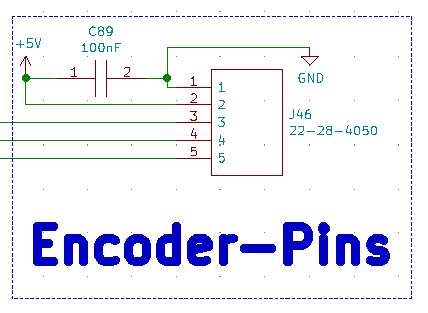
\includegraphics[width=0.5\textwidth]{graphics/Schema_ABN_Encoder}
%	\caption{Schema ABN-Encoder.}
%	\label{fig:Schema_ABN_Encoder}
%\end{figure} 